% Predlozak za pisanje diplomskog rada na PMF-MO
% Opcenita uputstva za LaTeX se mogu npr. naci na 
% http://web.math.hr/nastava/rp3, http://web.math.hr/nastava/s4-prof/latex.pdf
% NE PREPORUCA se "Ne baš tako kratak uvod u TEX", buduci se radi o vrlo starom prirucniku
% koji nije pogodan za moderne verzije LaTEXa.
% Originalna verzija "The not so short..." na http://tobi.oetiker.ch/lshort/lshort.pdf 
% je obnovljena i daje bolji uvid u moderne verzije LaTeXa

% Stil je optimiziran za kreiranje pdf dokumenta (npr. pomocu pdflatex-a, XeLaTeX-a)

\documentclass[a4paper,twoside,12pt]{memoir} % jednostrano: promijeniti twoside u oneside

% Paket inputenc omogucava direktno unosenje hrvatskih dijakritickih znakova 
% opcija utf8 za unicode (unix, linux, mac)
% opcija cp1250 za windowse
\usepackage[utf8]{inputenc}  % ukoliko se koristi XeLaTeX onda je \usepackage{xunicode}\usepackage{xltxtra}

% Stil za diplomski, unutra je ukljucena podrska za hrvatski jezik
\usepackage{diplomski}
\usepackage{datetime}

% bibliografija na hrvatskom
\usepackage[languagenames,fixlanguage,croatian]{babelbib} % zahtijeva datoteku croatian.bdf
% hiperlinkovi 
\usepackage[pdftex]{hyperref} % ukoliko se koristi XeLaTeX onda je \usepackage[xetex]{hyperref}

% Odabir familije fontova:
% koristenjem XeLaTeX-a mogu se koristiti svi fontovi instalirani na racunalu, npr
% \defaultfontfeatures{Mapping=tex-text}
% \setmainfont[Ligatures={Common}]{Hoefler Text}
% ili
% \newcommand{\nas}[1]{\fontspec{Adobe Garamond Pro}\fontsize{24pt}{24pt}\color{Chocolate}\selectfont #1}
% i onda \nas{Naslov ...}
\usepackage{txfonts} % times new roman 

% Paket graphicx sluzi za manipuliranje grafikom 
\usepackage[pdftex]{graphicx} % ukoliko se koristi XeLaTeX onda je \usepackage[xetex]{graphicx}
% Paket amsmath je vec ukljucen
% Dodatno definirane matematicke okoline:
% teorem (okolina: thm), lema (okolina: lem), korolar (okolina: cor),
% propozicija (okolina: prop), definicija (okolina: defn), napomena (okolina: rem),
% slutnja (okolina: conj), primjer (okolina: exa), dokaz (okolina: proof)
% Definirane su naredbe za ispisivanje skupova N, Z, Q, R i C
% Definirane su naredbe za funkcije koje se u hrvatskoj notaciji oznacavaju drukcije 
% nego u americkoj: tg, ctg, ... (\tgh za tangens hiperbolni)
% Takodjer su definirane naredbe za Ker i Im (da bi se razlikovala od naredbe za imaginarni dio kompleksnog
% broja, naredba se zove \slika).
\newdateformat{monthyeardate}{%
  \monthname[\THEMONTH], \THEYEAR}

\pagestyle{headings}
% uz paket fancyhdr mogu se lako kreirati fancy zaglavlja i podnozja

% Podaci koje treba unijeti
\title{RaČunanje rezonantnih modova u susatavu BEM++}
\author{Marko Dominković}
\advisor{Luka Grubišić}  % obavezno s titulom (prof. dr. sc ili doc. dr. sc.)
\date{\monthyeardate\today}  % oblika mjesec, godina

% Moguce je unijeti i posvetu
% Ukoliko nema posvete, dovoljno je iskomentirati/izbrisati sljedeci redak 
\dedication{Samom sebi}

\begin{document}

% Naredna frontmatter generira naslovnu stranicu, stranicu za potpise povjerenstva, eventualnu posvetu i sadrzaj
% Moze se iskomentirati ukoliko nije u pitanju konacna verzija
\frontmatter

% Tekst diplomskog ...

% Diplomski rad treba poceti s uvodnim poglavljem  
\begin{intro}
U ovom radu ćemo implementirat metodu za rješavanje problema računanja rezonatnih modova u problemu akustičkog ili elektromagnetskog raspršenja. Za rješavanje danih problema koristit ćemo BEM++ sustav.    
\end{intro}

\chapter{Rezonance i modovi}	
Sustav 
\begin{equation}
\label{eq:Af=0}
(I+A(w))f_{0}=0
\end{equation}
ima netrijvijalno rješenje za $f_0$ samo ako operator $(I+A(w))^{-1}$ je singularan za određenu frekvenciju $w$.

\chapter{BEM++}	
\section{O BEM++}

\cite{bempp} Bem++ je sustav za rješavanje akustičnih, elektrostatičkih i elektromagnetnih problema pomoću metode rubnih elemenata (boundary element method). Moguće ga je koristiti kroz sučelja programskih jezika Python i C\texttt{++}.

\section{Primjena BEM++}
\subsection{Rešetke i funkcijski prostori}
Za prikaz oblika nekog tijela u BEM++ koristimo se rešetkama. Rešetka je skup točaka u prostoru (dvodimenzionalnom ili trodimenzionalnom) i skup bridova koji povezuju... Konstruirajmo jednu jednostavnu rešetku \\
\hrule
\begin{lstlisting}[language=Python]
import bempp.api
import numpy as np

grid = bempp.api.shapes.regular_sphere(3)
\end{lstlisting}
\hrule 
\vspace{1cm}
Drugi način konstruiranja rešetke je pomoću polja vrhova i elemenata koji opisuju kako su vrhovi povezani. Sa \texttt{vertices} označimo polje svih vrhova. \texttt{evaluation\_points} opisuje način na koji su ovrhovi povezani.  \\
\hrule
\begin{lstlisting}[language=Python]
vertices = np.array([[0,1,2,1],
                     [0,2,0,1],
                     [0,0,0,2]])
                     
evaluation_points = np.array([[0,0,0,1],
                              [1,1,2,2],
                              [2,3,3,3]])
                              
grid = bempp.api.grid_from_element_data(vertice, evaluation_points)
\end{lstlisting} 
\hrule
\vspace{1cm}
Prvi element povezuje vrhove 0, 1 i 2. Drugi povezuje 0, 1 i 3 itd. 
Rešetke možemo učitati iz .msh datoteka. BEM++ podržava Gmsh v2.2 msh format
\begin{lstlisting}[language=Python]                                                       
grid = bempp.api.import_grid('my_grid.msh')
\end{lstlisting}
Važnu ulogu u BEM++ imaju funkcijski prostori. Za inicijalizaciju funkcijskog prostora potrebna nam je rešetka. 
\begin{lstlisting}[language=Python]                                                       
space = bempp.api.function_space(grid, "P", 0)
\end{lstlisting} 
Prvi argument funkcije je rešetka. Drugi argument je tip prosotra, u ovom slučaju \texttt{"P"} označava  prostor polinoma. 

\subsection{Operatori}
Operator $A$ difiniramo kao $$A:\mathcal{D} \rightarrow \mathcal{R}$$ preslikavanje s domene $D$ na kodomenu $R$, gdje su $D$ i $R$ definirane na površini dane rešetke. BEM++ ne koristi s direktno rubnim operatorom $A$, već slabijom formom 
\begin{equation}
a(u,v):=\int_\Gamma[Au](\mathbf{y})\overline{v(\mathbf{y})}d\mathbf{y},\quad u\in \mathcal{D}, v\in \mathcal{V}
\end{equation}  
gdje je $\mathcal{V}$ dualni prostor prostora $\mathcal{R}$. Rubni operatori se nalaze u paketu \newline \texttt{bempp.api.operators.boundary}. Neka je $g(x,y)$ Greenova funkcija. Definiramo jednoslojni $\mathcal{V}$ i dvoslojni $\mathcal{K}$ potencijalni operator sa:
\begin{equation}
[\mathcal{V}\Phi](\mathbf{x})=\int_\Gamma g(\mathbf{x},\mathbf{y})\Phi(\mathbf{y})ds(\mathbf{y}), \quad \mathbf{x}\in \mathbb{R}^{3}\backslash \Gamma
\end{equation}
\begin{equation}
[\mathcal{K}\Phi](\mathbf{x})=\int_\Gamma \frac{\partial g(\mathbf{x},\mathbf{y})}{\partial v(\mathbf{y})}g(\mathbf{x},\mathbf{y})\Phi(\mathbf{y})ds(\mathbf{y}), \quad \mathbf{x}\in \mathbb{R}^{3}\backslash \Gamma
\end{equation}
Sada iz njih izvodimo sljedeće granične operatore:

\begin{table}[H]
\begin{tabular}{m{7cm} m{7cm}}
\large{Operator} & \large{Formula} \\ \hline \\
 Jednoslojni rubni operator & $[V\phi](x)=\int_\Gamma g(\mathbf{x},\mathbf{y})\phi(\mathbf{y})d\mathbf{y},\quad \mathbf{x}\in \Gamma$ \\ \\ \hline \\
Dvoslojni rubni operator & $[K\phi](\mathbf{x})=\int_\Gamma\frac{\partial g(\mathbf{x},\mathbf{y})}{\partial v(\mathbf{y})}\phi(\mathbf{y})d\mathbf{y}, \quad \mathbf{x}\in \Gamma$ \\\\ \hline \\
Adjungirani dvoslojni rubni operator & $[K^{'}\phi](\mathbf{x})=\int_\Gamma\frac{\partial g(\mathbf{x},\mathbf{y})}{\partial v(\mathbf{y})}\phi(\mathbf{y})d\mathbf{y}, \quad \mathbf{x}\in \Gamma$ \\\\ \hline \\
 Hipersingularni rubni operatori& $[D\phi](x)=-\frac{\partial}{\partial v(\mathbf{x})}\int_\Gamma \frac{\partial g(\mathbf{x},\mathbf{y})}{\partial v(\mathbf{y})}\phi(\mathbf{y})d\mathbf{y}, \quad \mathbf{x} \in \Gamma$
\end{tabular}
\end{table}

 Dostupni operator s obzirom na odabir Greenove funkcije su:
\begin{table}[H]
\begin{tabular}{m{2.5cm} m{3cm} m{8cm}}\\
\large{PDJ} & \large{Greenova funkcija} & \large{Modul} \\
\hline
Laplace $-\Delta u=0$ & $g(x,y)=\frac{1}{4\pi|x-y|}$ & \texttt{bempp.api.operators.boundary,laplace}\\
\hline
Helmholtz $\Delta u+k^{2}u=0$ & $g(x,y)=\frac{e^{ik|x-y|}}{4\pi|x-y|}$ & \texttt{bempp.api.operators.boundary.helmholtz} \\
\hline
Modified \newline Helmholtz $-\Delta u + w^{2}u=0$ & $g(x,y)=\frac{e^{-w|x-y|}}{4\pi|x-y|}$ & \texttt{bempp.api.operators.boundary.modified\_helmholtz}
\end{tabular}
\end{table}
Svi rubni operatori su definirani sa domenom, kodomenom i dualni prostorom kodomene. U BEM++ se implementiraju na sljedeći naći:\\

\hrule
\begin{lstlisting}[language=Python]
grid = bempp.api.shapes.regular_sphere(3)
space = bempp.api.function_space(grid, "DP", 0)
slp = bempp.api.operators.boundary.laplace.
      single_layer(space, space, space)
\end{lstlisting}
\hrule

\subsection{Rješavanje linearnih jednadžbi}

Promotrimo sljedeći primjer $$A\phi=f $$  gdje su $f$ i $\phi$ funkcijske mreže. Zadanu jednadžbu možemo zapisati u njezinoj slabijoj formi: $$<Au,v>=<f,v>$$ za sve $v$ u dualnom prostoru. Uobičajni način rješavanje ovakvog sustava u Bempp je sljedeći:
\begin{enumerate}
	\item{ Izračunati slabu formu od $A$ pomoću 
	\begin{lstlisting} [language=Python]
	A_discrete = A.weak_form()
	\end{lstlisting}
	}
	\item{ Računanje projekcije $f$ na dualni prostor 
	\begin{lstlisting} [language=Python]
	p = f.projections(A.)
	\end{lstlisting}}
	\item{
	Pomoću funkcije \texttt{gmres}, iz SciPy paketa, riješimo sustav 
	\begin{lstlisting} [language=Python]
	x, info = gmres(discrete_op, p)
	\end{lstlisting}
	}
	\item{
	Iz rezultata \texttt{x} konstruirajmo funkcijsku mrežu sa
	\begin{lstlisting} [language=Python]
phi = bempp.api.GridFunction(A.domain, coefficients=x)
	\end{lstlisting}
	}
	
\end{enumerate}
  

\chapter{}

\section{Računanje najmanje svojstvene vrijednosti}

Neka je $A \in M_n$ kvadratna matrica reda $n$, $n\in \mathbb{N}$. Najmanja svojstvena vrijednost matrice $A$ ujedno je i najveća svojstvena vrijednost matrice $A^{-1}$. Najveća svojstvena vrijednost može se izračunati iterativnom metodom. Opišimo iterativnu metodu za dani matricu $A$. Za početak odaberimo vektor $b_0 \in \mathbb{R}^{n}$. Definirajmo niz $(b_n)$ na sljedeći način: $$b_{k+1}=\frac{Ab_k}{||Ab_k||},\quad k \in \mathbb{N}$$ Navedeni niz konvergira prema svojstvenom vektoru $x \in \mathbb{R}^n$ čija je odogovarajuća svojstvena vrijednost $\lambda$ najveća svojstvena vrijednost matrice $A$.
Za računanje najmanje svojstvene vrijednosti treba izračunati inverz matrice $A$,  $A^{-1}$, s pretpostavkom da je matrica $A$ regularna. Pritom primjenimo iterativnu metodu sa $A^{-1}$. Naravno, time se složenost samog algortima povećava. Druga mogučnost je rješavanje jednadžbe
\begin{equation}
\label{eq:Ax=b}
	Ax=b
\end{equation}
 u svakoj od iteraciji, gdje je $A \in M_n$, a $b \in \mathbb{R}^n$. Broj iteracija ovisi o izboru početnog vektora i točnosti koju želimo postići. Svojstvena vrijednost jednaka je inverzu norme svojstvenog vektora, $\lambda=1/||x||$. Opišimo algoritme za računanje najmanje singularne vrijednosti matrice $A$.\newpage
Prvi aloritam je modificirani oblik iterativne metode u kojem imamo z \\

\begin{algorithm}[H]
\SetAlgoLined
\SetKwInOut{Input}{Ulaz}
\SetKwInOut{Output}{Izlaz}
\Input{Regularna kvadratna matrica A veličine $n\times n$}
\Output{Najmanja singularna vrijednost}
 	$b=$ slučajni vektor \;
 	$e = 0.0001$ (točnost)\;
 	$razlika = 1$\;
 	\While{razlika $\geq$ e}{
 	riješi jednandžbu $Ax=b$\;
 	$x={x}/{||x||}$\;
 	$razlika=||b-x||$\;
 	$b=x$\;
 	}
 	\Return $1/||x||$
 \caption{Najmanja singularna vrijednost }
\end{algorithm}

U drugom algoritmu najprije izračunamo inverz matrice $A$ pa potom provodimo klasični iterativi algoritam za traženje najveće svojstvene vrijednosti.\\

\begin{algorithm}[H]
\SetAlgoLined
\SetKwInOut{Input}{Ulaz}
\SetKwInOut{Output}{Izlaz}
\Input{Regularna kvadratna matrica A veličine $n\times n$}
\Output{Najmanja singularna vrijednost}
 	$b=$ slučajni vektor,  $e = 0.0001$ (točnost), $razlika = 1$\;
 	$A_{inverz}=A^{-1}$ \;
 	\While{razlika $\geq$ e}{
 		$x=A_{inverz}b$\;
 		$x={x}/{||x||}$\;
 		$razlika=||b-x||$\;
 		$b=x$\;
 	}
 	\Return $1/||x||$
 \caption{Najmanja singularna vrijednost: inverz matrice }
\end{algorithm}
\newpage

Koji od navedenih algoritama je bolji? Naime, složenost rješavanja sustava $Ax=b$, gdje je $A$ matrica veličine $n \times n$, je $O(n^{3})$. Isto tako, računanje inverza matrice $A$ je složenosti $O(n^{3})$. Prednost ovog načina je ta da se inverz matrice izračuna samo jednom u odnosu na prvi alogritam, gdje se prilikom svake od iteracije rješava sustav ~\ref{eq:Ax=b}. Broj iteracija je ve



\chapter[Naslov poglavlja u sadržaju][Kratki naslov poglavlja]{Naslov poglavlja}	
% ukoliko naslov nije jako dugacak dovoljno je samo \chapter{Naslov poglavlja} 

\section[Naslov sekcije u sadržaju][Kratki naslov sekcije]{Naslov sekcije}
\subsection{Naslov podsekcije}
\begin{thm}
Iskaz teorema u kojem se javljaju skupovi  $\N$, $\Z$, $\Q$, $\R$ i $\C$.
\end{thm}
\begin{conj}
Iskaz slutnje u kojoj se javljaju funkcije $\tg$, $\tgh$ i $\sh$.
\end{conj}
\begin{cor}
Iskaz posljedice u kojoj se javljaju skupovi $\Ker T$ i $\slika T$..
\end{cor}
\begin{proof}
Dokaz posljedice se nalazi u \cite{kljuc}. Pogledajte i \cite{kurepa1956convex}, \cite{kurepa1981funkcionalna} te \cite{bempp}.
\end{proof}
jsfdsqF
SG
SFG
FSG
DF
GS
FG
SFG
SFG

SFG

SG
SDFG
SF
GS

DG
 SD
S


SD
 

DFGSDFG


SDGSDF


SDGSDGF


SDGFSFDG


SDGSDG  sdfsfg f fdh fgj gh jgjk jkj k yk k klk l fs fd gsdfg dfh dfghj fj ghjk gjk jlk sdf 
$x_1+x_2+x_3+x_4=12$ $x_1+x_2+x_3+x_4=12$
 $x_1+x_2+x_3+x_4=12$ $x_1+x_2+x_3+x_4=12$ $x_1+x_2+x_3+x_4=12$ $x_1+x_2+x_3+x_4=12$
 $x_1+x_2+x_3+x_4=12$ $x_1+x_2+x_3+x_4=12$ $x_1+x_2+x_3+x_4=12$
$x_1+x_2+x_3+x_4=12$ 
SDGSG sdfsfg f fdh fgj gh jgjk jkj k yk k klk l fs fd gsdfg dfh dfghj fj ghjk gjk jlk sdf sfdh j fj tuk ugad h j yrtu iru i
\[ z \left( 1 \ +\ \sqrt{\omega_{i+1} + \zeta -\frac{x+1}{\Theta +1} y + 1}
\ \right) =  1 \]

GSDFGSDFG



\begin{equation}
\label{eq:jed1}
	1+1=2
\end{equation}

dasdsa
SDFGS

SDFGSFG


SFGSFG


SDFGSFG


SDGSFG

\label{stranica}
Na stranici \pageref{stranica} se nalaza slika u \textbf{png} formatu.
% slike smiju biti u svim formatima koje podrzava pdf (pdf, jpg, png)
\begin{figure}[h!t]
\begin{center}

\includegraphics[scale=0.5]{mosaic-from-pompeii.png}
\caption{Prva slika}
\end{center}
\end{figure}

Na slici \ref{fig:3d} se nalazi 3D graf neke funkcije. 

\begin{figure}[h!t]
\centering 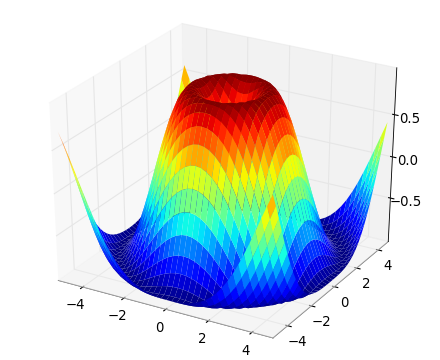
\includegraphics{surface3d.png}
\caption{Druga slika}
\label{fig:3d}
\end{figure}

kao i jedna vrlo komplicirana formula koja slijedi iz \eqref{eq:jed1}
\[ \sum_{i=1}^{\infty}A_{x_1}\times A_{{\alpha}_2}\oslash\iint_{\Omega}x^2\ddagger\limsup_{n\in\N}\frac{\alpha+\theta+\gamma}{n^{\omega}}\;\;\text{je u stvari}\;\;\biguplus_{r\in\Q}\overline{\Xi_i \mathop\Theta_{\substack{j\in\C \\ j\ni i\Q}} \Upsilon^{k^j} \underset{\ast}{\Psi} \hslash\vert_{\{\alpha\}}}.\]

% Na kraju diplomkog rada stavlja se  bibliografija
% Najprije definiramo nacin prikazivanja bibliografije, u ovom slucaju verzija amsplain stila
\bibliographystyle{babamspl} % babamspl ili babplain

% U datoteku diplomski.bib se stavljaju bibliografske reference
% Bibliografske reference u bib formatu se mogu dobiti iz MathSciNet baze, Google Scholara, ArXiva, ...
\bibliography{diplomski}

\pagestyle{empty} % ne zelimo brojanje sljedecih stranica

% I na koncu idu sazeci na hrvatskom i engleskom

\begin{sazetak}
CDSADAS dasd asd as
\end{sazetak}

\begin{summary}
In this ...
\end{summary}

% te zivotopis

\begin{cv}
Dana ...
\end{cv}

\end{document}